\chapter{Differential forms}
In this chapter, all vector spaces are finite-dimensional
real inner product spaces.
We first start by (non-rigorously) drawing pictures
of all the things that we will define in this chapter.
Then we re-do everything again in its proper algebraic context.

\section{Pictures of differential forms}
Before defining a differential form,
we first draw some pictures.
The key thing to keep in mind is
\begin{moral}
	``The definition of a differential form is:
	something you can integrate.'' \\ --- Joe Harris
\end{moral}

We'll assume that all functions are \vocab{smooth},
i.e.\ infinitely differentiable.

Let $U \subseteq V$ be an open set of a vector space $V$.
Suppose that we have a function $f : U \to \RR$, i.e.\
we assign a value to every point of $U$.
\begin{center}
	\begin{asy}
		bigblob("$U$");
		dot("$3$", (-2,1), red);
		dot("$\sqrt2$", (-1,-1), red);
		dot("$-1$", (2,2), red);
		dot("$0$", (-3,-3), red);
	\end{asy}
\end{center}
\begin{definition}
	A \vocab{$0$-form} $f$ on $U$ is just a smooth function $f : U \to \RR$.
\end{definition}
Thus, if we specify a finite set $S$ of points in $U$
we can ``integrate'' over $S$ by just adding up the values
of the points:
\[ 0 + \sqrt 2 + 3 + (-1) = 2 + \sqrt2. \]
So, \textbf{a $0$-form $f$ lets us integrate over $0$-dimensional ``cells''}.

But this is quite boring, because as we know we like
to integrate over things like curves, not single points.
So, by analogy, we want a $1$-form to let us integrate
over $1$-dimensional cells: i.e.\ over curves.
What information would we need to do that?
To answer this, let's draw a picture of a curve $c$,
which can be thought of as a function $c : [0,1] \to U$.
\begin{center}
	\begin{asy}
		bigblob("$U$");
		pair a = (-2,-2);
		pair b = (3,0);
		pair p = (0,1);
		pair q = (2,0);
		label("$c$", q, dir(45), heavygreen);
		dot(a, heavygreen);
		dot(b, heavygreen);
		draw(a..p..q..b, heavygreen);
		dot("$p$", p, dir(90), blue);
		pair v = p+1.5*dir(-10);
		label("$v$", v, dir(50), blue);
		draw(p--v, blue, EndArrow);
	\end{asy}
\end{center}
We might think that we could get away
with just specifying a number on every point of $U$
(i.e.\ a $0$-form $f$), and then somehow ``add up''
all the values of $f$ along the curve.
We'll use this idea in a moment, but we can in fact do something more general.
Notice how when we walk along a smooth curve, at every point $p$
we also have some extra information: a \emph{tangent vector} $v$.
So, we can define a $1$-form $\alpha$ as follows.
A $0$-form just took a point and gave a real number,
but \textbf{a $1$-form will take both a point \emph{and} a tangent
vector at that point, and spit out a real number.}
So a $1$-form $\alpha$ is a smooth function on pairs $(p,v)$,
where $v$ is a tangent vector at $p$, to $\RR$.  Hence
\[ \alpha : U \times V \to \RR. \]

Actually, for any point $p$, we will require that $\alpha(p,-)$
is a linear function in terms of the vectors:
i.e.\ we want for example that $\alpha(p,2v) = 2\alpha(p,v)$.
So it is more customary to think of $\alpha$ in the following way:
\begin{definition}
	A \vocab{$1$-form} $\alpha$ is a smooth function
	\[ \alpha : U \to V^\vee. \]
\end{definition}
Like with $Df$, we'll use $\alpha_p$ instead of $\alpha(p)$.
So, at every point $p$, $\alpha_p$ is some linear functional
that eats tangent vectors at $p$, and spits out a real number.
Thus, we think of $\alpha_p$ as an element of $V^\vee$;
\[ \alpha_p \in V^\vee. \]

Next, we draw pictures of $2$-forms.
This should, for example, let us integrate over a blob
(a so-called $2$-cell) of the form
\[ c : [0,1] \times [0,1] \to U \]
i.e.\ for example, a square in $U$.
In the previous example with $1$-forms,
we looked at tangent vectors to the curve $c$.
This time, at points we will look at \emph{pairs} of tangent vectors
in $U$: in the same sense that lots of tangent vectors
approximate the entire curve, lots of tiny squares
will approximate the big square in $U$.
\begin{center}
	\begin{asy}
		bigblob("$U$");
		filldraw( (-2,-2)--(-2,2)--(2,2)--(2,-2)--cycle, 
			opacity(0.4) + orange, red);
		label("$c$", (2,2), dir(45), red);
		for (real t = -1; t < 2; t += 1) {
			draw( (-2,t)--(2,t), red );
			draw( (t,-2)--(t,2), red );
		}
		pair p = (-1, -1);
		dot("$p$", p, dir(225), blue);
		pair v = p + dir(90);
		pair w = p + dir(0);
		draw(p--v, blue, EndArrow);
		draw(p--w, blue, EndArrow);
		label("$v$", v, dir(135), blue);
		label("$w$", w, dir(-45), blue);
	\end{asy}
\end{center}
So what should a $2$-form $\beta$ be?
As before, it should start by taking a point $p \in U$,
so $\beta_p$ is now a linear functional:
but this time, it should be a linear map on two vectors $v$ and $w$.
Here $v$ and $w$ are not tangent so much as their span cuts out
a small parallelogram. So, the right thing to do is in fact consider
\[ \beta_p \in V^\vee \wedge V^\vee. \]
That is, to use the wedge product to get a handle on
the idea that $v$ and $w$ span a parallelogram.
Another valid choice would have been $(V \wedge V)^\vee$;
in fact, the two are isomorphic, but it will be more convenient
to write it in the former.

\section{Pictures of exterior derivatives}
Next question:
\begin{moral}
	How can we build a $0$-form from a $1$-form?
\end{moral}
Let $f$ be a $0$-form on $U$; thus, we have a function $f : U \to \RR$.
Then in fact there is a very natural $1$-form on $U$ arising
from $f$, appropriately called $df$.
Namely, given a point $p$ and a tangent vector $v$,
the differential form $(df)_p$ returns the \emph{change in $f$ along $v$}.
In other words, it's juts the total derivative $(Df)_p(v)$.
\begin{center}
	\begin{asy}
		bigblob("$U$");
		dot("$3$", (-2,1), red);
		dot("$\sqrt2$", (-1,-1), red);
		dot("$-1$", (2,2), red);
		dot("$0$", (-3,-3), red);
		draw((-1,-1)--(0,1), blue, EndArrow);
		label("$\sqrt2 + \varepsilon$", (0,1), dir(90), blue);
		label("$v$", (-0.5, 0), dir(0), blue);
	\end{asy}
\end{center}
Thus, $df$ measures ``the change in $f$''.

Now, even if I haven't defined integration yet,
given a curve $c$ from a point $a$ to $b$, what do you think
\[ \int_c df \]
should be equal to?
Remember that $df$ is the $1$-form that measures
``infinitesimal change in $f$''.
So if we add up all the change in $f$ along a path from $a$ to $b$,
then the answer we get should just be
\[ \int_c df = f(b) - f(a). \]
This is the first case of something we call Stokes' theorem.

Generalizing, how should we get from a $1$-form to a $2$-form?
At each point $p$, the $2$-form $\beta$ gives a $\beta_p$
which takes in a ``parallelogram'' and returns a real number.
Now suppose we have a $1$-form $\alpha$.
Then along each of the edges of a parallelogram,
with an appropriate sign convention the $1$-from $\alpha$ gives
us a real number.
So, given a $1$-form $\alpha$, we define $d\alpha$
to be the $2$-form that takes in a parallelogram
spanned by $v$ and $w$,
and returns \textbf{the measure of $\alpha$ along the boundary}.

Now, what happens if you integrate $df$ along the entire square $c$?
The right picture is that, if we think of each little square
as making up the big square, then the adjacent boundaries cancel out,
and all we are left is the main boundary.
This is again just a case of the so-called Stokes' theorem.

\begin{center}
	\begin{asy}
		bigblob("$U$");
		filldraw( (-2,-2)--(-2,2)--(2,2)--(2,-2)--cycle, 
			opacity(0.4) + orange, red);
		label("$c$", (2,2), dir(45), red);
		for (real t = -1; t < 2; t += 1) {
			draw( (-2,t)--(2,t), red );
			draw( (t,-2)--(t,2), red );
		}
		pair p = (-1, -1);
		dot("$p$", p, dir(225), blue);
		pair v = p + dir(90);
		pair w = p + dir(0);
		pair x = w + v - p;
		draw(p--w, blue, EndArrow);
		draw(w--x, blue, EndArrow);
		draw(x--v, blue, EndArrow);
		draw(v--p, blue, EndArrow);
	\end{asy}
	\hspace{4em}
	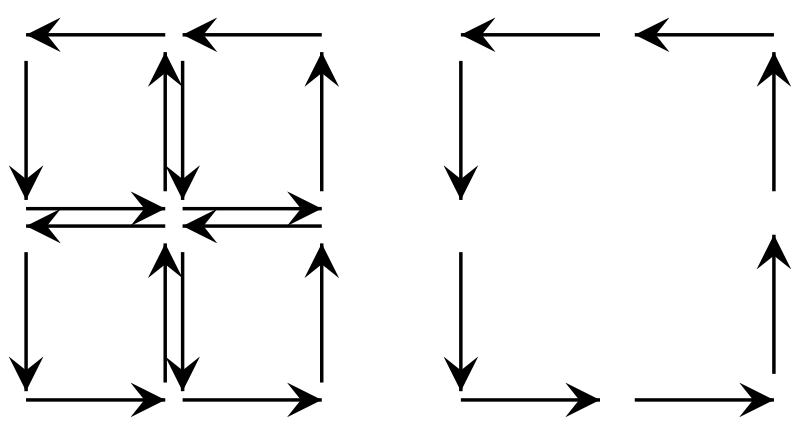
\includegraphics[width=6cm]{media/stokes-patch.png}
\end{center}


\section{Differential forms}
\prototype{Algebraically,
	something that looks like $f \ee_1^\vee \wedge \ee_2^\vee + \dots$,
	and geometrically, see the previous section.}

Let's now get a handle on what $dx$ means.
Fix a real vector space $V$ of dimension $n$,
and let $\ee_1$, \dots, $\ee_n$ be a standard basis.
Let $U$ be an open set.

\begin{definition}
	We define a \vocab{differential $k$-form} $\alpha$ on $U$
	to be a smooth (infinitely differentiable) map
	$\alpha : U \to \Lambda^k(V^\vee)$.
	(Here $\Lambda^k(V^\vee)$ is the wedge product.)
\end{definition}

Like with $Df$, we'll use $\alpha_p$ instead of $\alpha(p)$.

\begin{example}
	[$k$-forms for $k=0,1$]
	\listhack
	\begin{enumerate}[(a)]
		\item A $0$-form is just a function $U \to \RR$.
		\item A $1$-form is a function $U \to V^\vee$.
		For example,
		the total derivative $Df$ of a function $V \to \RR$ is a $1$-form.
		\item Let $V = \RR^3$ with standard basis $\ee_1$, $\ee_2$, $\ee_3$.
		Then a typical $2$-form is given by
		\[
			\alpha_p
			=
			f(p) \cdot \ee_1^\vee \wedge \ee_2^\vee
			+ g(p) \cdot \ee_1^\vee \wedge \ee_3^\vee
			+ h(p) \cdot \ee_2^\vee \wedge \ee_3^\vee
			\in \Lambda^2(V)
		\]
		where $f,g,h : V \to \RR$ are smooth functions.
	\end{enumerate}
\end{example}

Now, by the projection principle (\Cref{thm:project_principle}) we only have to specify
a function on each of $\binom nk$ basis elements of $\Lambda^k(V^\vee)$.
So, take any basis $\{e_i\}$ of $V$, and 
take the usual basis for $\Lambda^k(V^\vee)$ of elements
\[ e_{i_1}^\vee \wedge e_{i_2}^\vee \wedge \dots \wedge e_{i_k}^\vee. \]
Thus, a general $k$-form takes the shape
\[ \alpha_p = \sum_{1 \le i_1 < \dots < i_k \le n} 
	f_{i_1, \dots, i_k}(p) \cdot
	e_{i_1}^\vee \wedge e_{i_2}^\vee \wedge \dots \wedge e_{i_k}^\vee. \]
Since this is a huge nuisance to write, we will abbreviate this to just
\[ \alpha = \sum_I f_I \cdot de_I \]
where we understand the sum runs over $I = (i_1, \dots, i_k)$,
and $de_I$ represents $e_{i_1}^\vee \wedge \dots \wedge e_{i_k}^\vee$.

Now that we have an element $\Lambda^k(V^\vee)$, what can it do?
Well, first let me get the definition on the table, then tell you what it's doing.
\begin{definition}
	For linear functions $\xi_1, \dots, \xi_k \in V^\vee$
	and vectors $v_1, \dots, v_k \in V$, set
	\[
		(\xi_1 \wedge \dots \wedge \xi_k)(v_1, \dots, v_k)
		\defeq
		\det
		\begin{bmatrix}
			\xi_1(v_1) & \dots & \xi_1(v_k) \\
			\vdots & \ddots & \vdots \\
			\xi_k(v_1) & \dots & \xi_k(v_k)
		\end{bmatrix}.
	\]
	You can check that this is well-defined
	under e.g. $v \wedge w = -w \wedge v$ and so on.
\end{definition}

\begin{example}
	[Evaluation of a differential form]
	Set $V = \RR^3$.
	Suppose that at some point $p$, the $2$-form $\alpha$ returns
	\[ \alpha_p = 2 \ee_1^\vee \wedge \ee_2^\vee + \ee_1^\vee \wedge \ee_3^\vee. \]
	Let $v_1 = 3\ee_1 + \ee_2 + 4\ee_3$ and $v_2 = 8\ee_1 + 9\ee_2 + 5\ee_3$.
	Then
	\[
		\alpha_p(v_1, v_2)
		=
		2\det \begin{bmatrix}
			3 & 1 \\ 8 & 9 \end{bmatrix}
		+
		\det \begin{bmatrix}
			3 & 4 \\ 8 & 5 \end{bmatrix}
		= 21.
	\]
\end{example}

What does this definition mean?
One way to say it is that
\begin{moral}
	If I walk to a point $p \in U$,
	a $k$-form $\alpha$ will take in $k$ vectors $v_1, \dots, v_k$
	and spit out a number, which is to be interpreted as a (signed) volume.
\end{moral}

Picture:
\begin{center}
	\begin{asy}
		bigblob("$U$");
		pair p = (-2,-2);
		dot("$p$", p, dir(225), red);
		pair p1 = p + 1.4*dir(120);
		pair p2 = p + 1.7*dir(10);
		draw(p--p1, red, EndArrow);
		draw(p--p2, red, EndArrow);
		label("$v_1$", p1, dir(p1-p), red);
		label("$v_2$", p2, dir(p2-p), red);
		label("$\alpha_p(v_1, v_2) \in \mathbb R$", p+dir(45)*3);
	\end{asy}
\end{center}

In other words, at every point $p$, we get a function $\alpha_p$.
Then I can feed in $k$ vectors to $\alpha_p$ and get a number,
which I interpret as a signed volume of the parallelpiped spanned by the $\{v_i\}$'s
in some way (e.g.\ the flux of a force field).
That's why $\alpha_p$ as a ``function'' is contrived to lie in the wedge product:
this ensures that the notion of ``volume'' makes sense, so that for example,
the equality $\alpha_p(v_1, v_2) = -\alpha_p(v_2, v_1)$ holds.

This is what makes differential forms so fit for integration.


\section{Exterior derivatives}
\prototype{Possibly $dx_1 = \ee_1^\vee$.}
We now define the exterior derivative $df$ that we gave
pictures of at the beginning of the section.
It turns out that the exterior derivative is easy to compute
given explicit coordinates to work with.

First, given a function $f : U \to \RR$,
we define 
\[ df \defeq Df = \sum_i f_i e_i^\vee \]
In particular, suppose $V = \RR^n$ and $f(x_1, \dots, x_n) = x_1$ (i.e.\ $f = \ee_1^\vee$). Then:
\begin{ques}
	Show that for any $p \in U$, \[ \left( d(\ee_1^\vee) \right)_p = \ee_1^\vee. \]
\end{ques}

\begin{abuse}
	Unfortunately, someone somewhere decided it would be a good idea to use ``$x_1$'' to denote $\ee_1^\vee$
	(because \emph{obviously}\footnote{Sarcasm.} $x_1$ means
	``the function that takes $(x_1, \dots, x_n) \in \RR^n$ to $x_1$'')
	and then decided that \[ dx_1 \defeq \ee_1^\vee. \]
	This notation is so entrenched that I have no choice but to grudgingly accept it.
	Note that it's not even right, since technically it's $(dx_1)_p = \ee_1^\vee$; $dx_1$ is a $1$-form.
	\label{abuse:dx}
\end{abuse}
\begin{remark}
	This is the reason why we use the notation $\frac{df}{dx}$ in calculus now:
	given, say, $f : \RR \to \RR$ by $f(x) = x^2$, it is indeed true that
	\[ df = 2x \cdot \ee_1^\vee = 2x \cdot dx \]
	and so by abuse of notation we write $df/dx = 2x$.
\end{remark}

More generally, we can define the \vocab{exterior derivative} in terms of our basis $e_1$, \dots, $e_n$ as follows:
if $\alpha = \sum_I f_I de_I$ then we set
\[ d\alpha \defeq \sum_I df_I \wedge de_I = \sum_I \sum_j \fpartial{f_I}{e_j} de_j \wedge de_I. \]
This doesn't depend on the choice of basis.

\begin{example}[Computing some exterior derivatives]
	Let $V = \RR^3$ with standard basis $\ee_1$, $\ee_2$, $\ee_3$.
	Let $f(x,y,z) = x^4 + y^3 + 2xz$.
	Then we compute
	\[ df = Df = (4x^3+2z) \; dx + 3y^2 \; dy + 2x \; dz. \]
	Next, we can evaluate $d(df)$ as prescribed: it is
	\begin{align*}
		d^2f &= (12x^2 \; dx + 2 dz) \wedge dx + (6y \; dy) \wedge dy
		+ 2(dx \wedge dz) \\
		&= 12x^2 (dx \wedge dx) + 4(dz \wedge dx) + 6y (dy \wedge dy) + 4(dx \wedge dz) \\
		&= 4(dz \wedge dx) + 4(dx \wedge dz) \\
		&= 0.
	\end{align*}
	So surprisingly, $d^2f$ is the zero map.
	Here, we have exploited \Cref{abuse:dx} for the first time,
	in writing $dx$, $dy$, $dz$.
\end{example}
And in fact, this is always true in general:
\begin{theorem}[Exterior derivative vanishes]
	\label{thm:dd_zero}
	Let $\alpha$ be any $k$-form.
	Then $d^2(\alpha) = 0$.
	Even more succinctly, \[ d^2 = 0. \]
\end{theorem}
The proof is left as \Cref{prob:dd_zero}.
\begin{exercise}
	Compare the statement $d^2 = 0$ to the geometric
	picture of a $2$-form given at the beginning of this chapter.
	Why does this intuitively make sense?
\end{exercise}

Here are some other properties of $d$:
\begin{itemize}
	\ii As we just saw, $d^2 = 0$.
	\ii It is bilinear; $d(c\alpha+\beta) = c \cdot d\alpha + d\beta$.
	\ii For a $k$-form $\alpha$ and $\ell$-form $\beta$, one can show that
	\[ d(\alpha \wedge \beta) = d\alpha \wedge \beta + (-1)^k (\alpha \wedge d\beta). \]
\end{itemize}
In fact, one can show that $df$ as defined in terms of bases above is
the \emph{unique} map sending $k$-forms to $(k+1)$-forms.
Actually, one way to define $df$ is to take as axioms the bulleted properties above
and then declare $d$ to be the unique solution to this functional equation.
In any case, this tells us that our definition of $d$
does not depend on the basis chosen.

Recall that $df$ measures the change in boundary.
In that sense, $d^2 = 0$ is saying something like
``the boundary of the boundary is empty''.
We'll make this precise when we see Stokes' theorem in the next chapter.

\section{Closed and exact forms}
Let $\alpha$ be a $k$-form.
\begin{definition}
	We say $\alpha$ is \vocab{closed} if $d\alpha = 0$.
\end{definition}
\begin{definition}
	We say $\alpha$ is \vocab{exact} if for some $(k-1)$-form $\beta$,
	$d\beta = 0$.  If $k = 0$, $\alpha$ is exact only when $\alpha = 0$.
\end{definition}
\begin{ques}
	Show that exact forms are closed.
\end{ques}

A natural question arises: are there closed forms
which are not exact?
Surprisingly, the answer to this question is tied to topology.
Here is one important example.

\begin{example}
	[The angle form]
	\label{ex:angle_form}
	Let $U = \RR^2 \setminus \{0\}$,
	and let $\theta(p)$ be the angle formed by the $x$-axis
	and the line from the origin to $p$.

	The $1$-form $\alpha : U \to (\RR^2)^\vee$ defined by
	\[ \alpha = \frac{-y \; dx + x \; dy}{x^2+y^2} \]
	is called the \vocab{angle form}:
	given $p \in U$ it measures the change in angle $\theta(p)$
	along a tangent vector.
	So intuitively, ``$\alpha = d\theta$''.
	Indeed, one can check directly that the angle form is closed.

	However, $\alpha$ is not exact: there is no global smooth
	function $\theta : U \to \RR$ having $\alpha$ as a derivative.
	This reflects the fact that one can actually perform
	a full $2\pi$ rotation around the origin, i.e.\ $\theta$
	only makes sense mod $2\pi$.
	Thus existence of the angle form $\alpha$ reflects
	the possibility of ``winding'' around the origin.
\end{example}

So the key idea is that the failure of a closed form to be exact
corresponds quite well with ``holes'' in the space:
the same information that homotopy and homology groups are trying to capture.
To draw another analogy, in complex analysis Cauchy-Gorsat
only works when $U$ is simply connected.
The ``hole'' in $U$ is being detected by the existence of a form $\alpha$.
The so-called de Rham cohomology will make this relation explicit.

\section\problemhead
\begin{problem}
	Show directly that the angle form
	\[ \alpha = \frac{-y \; dx + x \; dy}{x^2+y^2} \]
	is closed.
\end{problem}
  
\begin{problem}
	\label{prob:dd_zero}
	Establish \Cref{thm:dd_zero}, which states that $d^2 = 0$.
	\begin{hint}
		This is just a summation.
		You will need the fact that mixed partials are symmetric.
	\end{hint}
\end{problem}
